\section{Создание параметрической модели центроплана}

Для анализа влияния формы кессона на вес самолета и его аэродинамические характеристики была создана параметрическая модель, представляющая из себя упрощенную модель центроплана. В упрощенной модели кессон заменен коробом переменного прямоугольного сечения с перегородками. На него передаются нагрузки путем приложения аэродинамических нагрузок на упрощенную модель крыла -- короб постоянного прямоугольного сечения (Рис.\ref{fig:CurvedKessonPatran}). Материал всех панелей - алюминий, толщина каждой панели постоянна, панели без вырезов. Все остальные части самолёта опущены для простоты.  

\begin{figure}[ht]
\centering
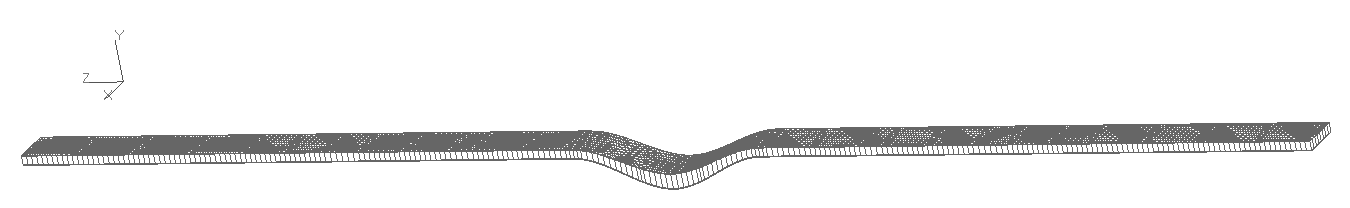
\includegraphics[width=0.9\textwidth]{CurvedKessonPatran}
\caption{Упрощенная модель центроплана}
\label{fig:CurvedKessonPatran}
\end{figure}

Для модели центроплана имеются два параметра: относительная координата нижней точки сечения и строительная высота в плоскости симметрии самолета. Кривые, описывающие нижнюю и верхнюю поверхность кессона выбраны кубическим сплайном через заданные исходя из параметров точки с условием равенства нулю производных в точках стыка фюзеляжа с крылом и в плоскости симметрии самолета (Рис.\ref{fig:KessSectionExample}).

\begin{figure}[ht]
\centering
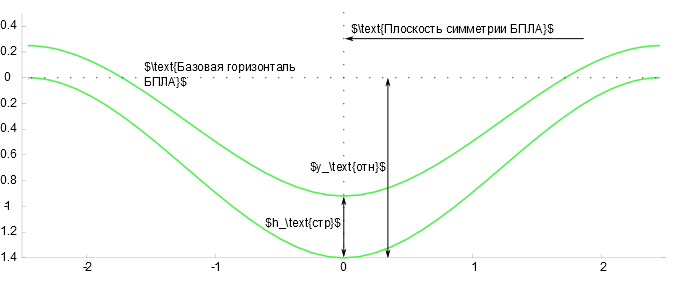
\includegraphics[width=0.5\textwidth]{KessSectionExample}
\caption{Пример модельного сечения центроплана}
\label{fig:KessSectionExample}
\end{figure}

Использование такой упрощенной модели в МКЭ-расчете позволяет ускорить процесс при тех же вычислительных мощностях. Так, в упрощенной модели используется $\approx10000$ конечных элементов, в то время как в полной модели самолета $\approx270000$ конечных элементов.

Так же, выбор такой параметрической модели позволит в дальнейшем включить в процесс оптимизации сечения так же расчет аэродинамических нагрузок, что позволит полностью автоматизировать процесс оптимизации формы сечения кессона для схемы "летающее крыло". 

